\Askhsh{18558}{2}
\begin{ylh}{1}
    \item 9.2. Το Πυθαγόρειο θεώρημα
    \item 10.3. Εμβαδόν βασικών ευθύγραμμων σχημάτων.
\end{ylh}
\begin{wrapfigure}[11]{r}{8cm}
    \centering
    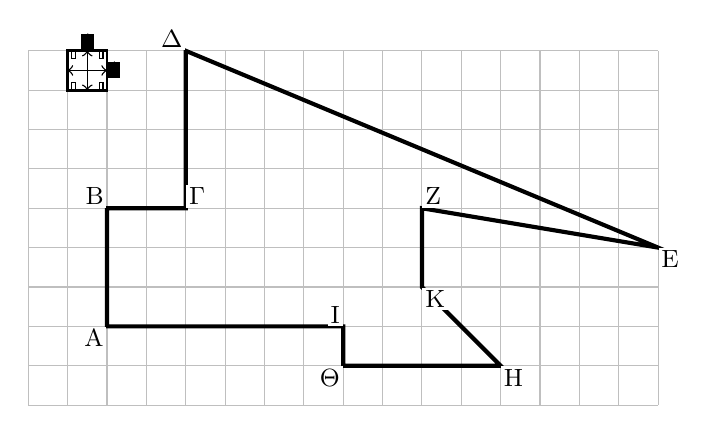
\begin{tikzpicture}[scale=0.5, every node/.style={font=\small, fill=white, inner sep=1pt}]
        % Draw the grid
        \draw[help lines, thin, gray!50] (0,0) grid (16,9);

        % Define points
        \coordinate (A) at (2,2);
        \coordinate (B) at (2,5);
        \coordinate (G) at (4,5); % Gamma
        \coordinate (D) at (4,9); % Delta
        \coordinate (E) at (16,4);
        \coordinate (Z) at (10,5);
        \coordinate (K) at (10,3);
        \coordinate (H) at (12,1);
        \coordinate (Th) at (8,1); % Theta
        \coordinate (I) at (8,2);

        % Draw the polygon
        \draw[line width=1.5pt, black] (A) -- (B) -- (G) -- (D) -- (E) -- (Z) -- (K) -- (H) -- (Th) -- (I) -- cycle;

        % Label the points
        \node[below left] at (A) {A};
        \node[above left] at (B) {B};
        \node[above right] at (G) {$\Gamma$};
        \node[above left] at (D) {$\Delta$};
        \node[below right] at (E) {E};
        \node[above right] at (Z) {Z};
        \node[below right] at (K) {K};
        \node[below right] at (H) {H};
        \node[below left] at (Th) {$\Theta$};
        \node[above left] at (I) {I};

        % Draw the small unit square
        \draw[line width=1pt] (1,8) rectangle (2,9);
        % Right angle symbols (small squares at corners)
        \draw (1.1,8) -- (1.1,8.2) -- (1.2,8.2) -- (1.2,8) -- cycle; % bottom left
        \draw (1.1,9) -- (1.1,8.8) -- (1.2,8.8) -- (1.2,9) -- cycle; % top left
        \draw (1.9,9) -- (1.9,8.8) -- (1.8,8.8) -- (1.8,9) -- cycle; % top right
        \draw (1.9,8) -- (1.9,8.2) -- (1.8,8.2) -- (1.8,8) -- cycle; % bottom right
        % Unit labels with arrows
        \draw[<->, line width=0.5pt, black] (1.0, 8.5) -- (2.0, 8.5) node[right, black, inner sep=0pt] {1};
        \draw[<->, line width=0.5pt, black] (1.5, 8.0) -- (1.5, 9.0) node[above, black, inner sep=0pt] {1};
    \end{tikzpicture}
\end{wrapfigure}
Στο παρακάτω σχήμα:
\begin{alist}
    \item Να βρείτε το μήκος της πλευράς $\Delta\text{E}$. \monades{10}
    \item Να υπολογίσετε το εμβαδόν του χωρίου που περικλείεται από την τεθλασμένη γραμμή $\text{AB}\Gamma\Delta\text{EZK H}\Theta\text{IA}$. \monades{15}
\end{alist}